% !TEX TS-program = LuaLaTeX
\documentclass[11pt,compress,xcolor=x11names,UTF8]{beamer}
\usetheme{Boadilla}
\usecolortheme{seahorse}
\useinnertheme[shadow]{rounded}  
\useoutertheme[subsection=false]{smoothbars}
\usecolortheme{spruce}
\usecolortheme[named=SpringGreen4]{structure}
\usefonttheme{structurebold}
\useinnertheme{circles}
\usecolortheme{rose}
\usepackage{pifont}
\usepackage{academicons}
\usepackage{fontawesome}
\usepackage{iitem}
\setbeamertemplate{itemize item}{\ding{108}}
\setbeamertemplate{itemize subitem}{\ding{109}}
\setbeamertemplate{navigation symbols}{}
\setbeamercovered{transparent}  
\renewcommand\appendixname{附录}
\renewcommand\abstractname{摘要}
\graphicspath{{figure/}} % 图片路径
\usepackage{calligra} % Thank you
\usepackage{ctex} % 加入中文
\setCJKsansfont{Noto Sans CJK SC}
\setsansfont{Lato} % Lato Roboto Fira Sans

\usepackage{url}					
\usepackage{natbib} % 参考文献
\title[Spatial Generalized Linear Mixed Models]{Spatial Generalized Linear Mixed Models with Application to Prevalence Mapping}
\subtitle{空间广义线性混合模型及其在预测流行病中的应用}
\author[黄湘云]{学生:黄湘云 \and 导师:李再兴 } % \\ 专业:统计学 \\ 方向:数据分析与统计计算
\institute[中国矿业大学(北京)]{理学院 \and 计算数学与统计系\and 2015级硕士学位论文答辩} % 理学院\\
\date[\today]{
\includegraphics[width=.5\textwidth]{logo}}

\begin{document}

\maketitle

\begin{frame}{Outline}
\tableofcontents
\end{frame}

\section{引言}

\subsection{研究意义}

\begin{frame}{例\emph{例} }
\textsf{例} \textbf{例}  \textit{例} 
% \texttt{例}  % 调出仿宋字体了

\begin{enumerate}
\item radionuclide concentrations on Rongelap Island
\item childhood malaria in the gambia
\item Loa loa prevalence in Cameroon and surrounding areas
\end{enumerate}

\end{frame}

\begin{frame}{Introduction}
\citet{Diggle2002}
\begin{itemize}
\item First item in the list
\item Second item
\item and so on
\begin{itemize}
\item First item in the list
\item Second item
\item and so on
\end{itemize}
\end{itemize}

\begin{itemize}
\item the effects of child level covariates (age and bed net use)
\item village level covariates (the primary health care and greenness of surrounding vegetation)
\item separate components for residual spatial
\item non-spatial extrabinomial variation
\end{itemize}
$\mathbb{R}^{n}$
$$ \mathsf{\log} \{p_{ij}/(1-p_{ij})\} =\alpha + \beta'z_{ij} + U_{i} + S(x_{i})$$

\end{frame}

\subsection{文献综述}

\begin{frame}
\begin{figure}
\centering
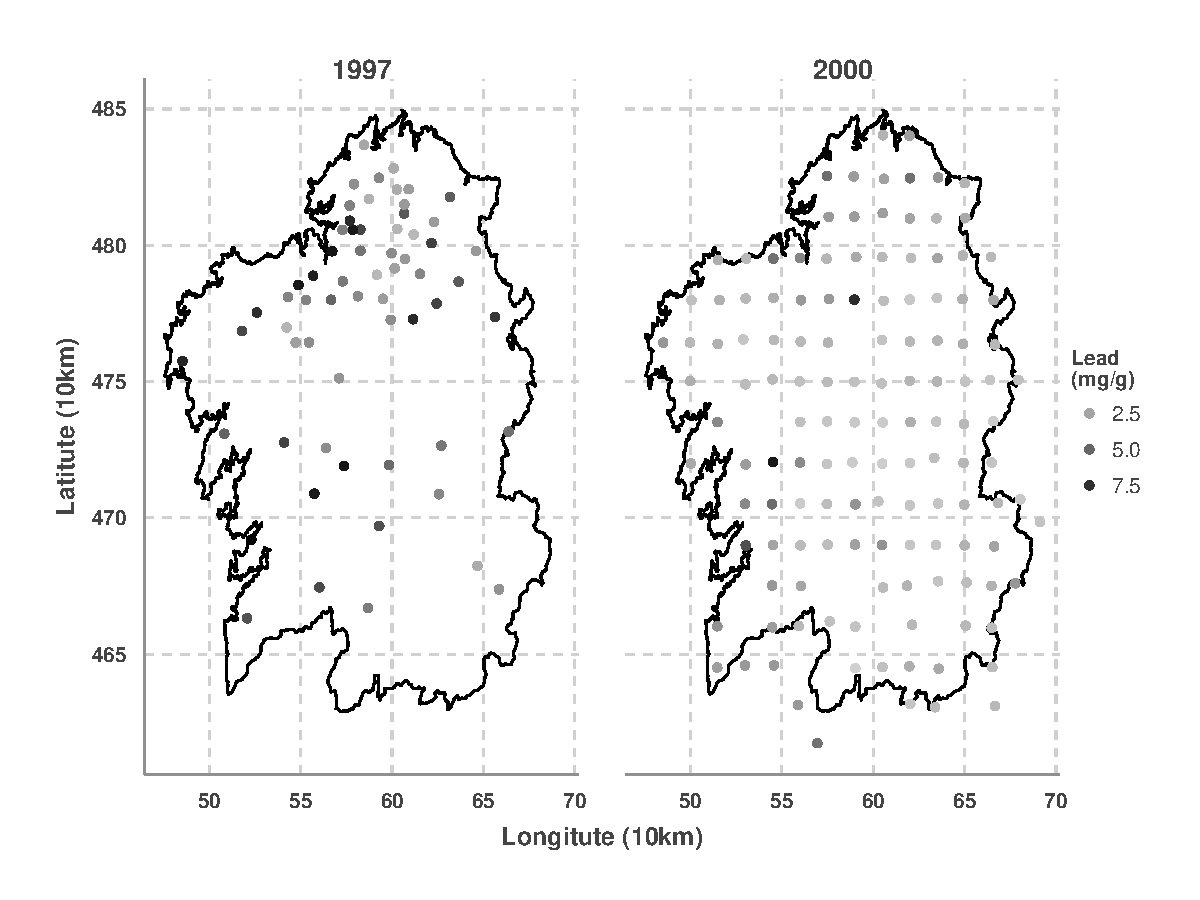
\includegraphics[width=.8\textwidth]{demo04}  
\end{figure}
\end{frame}

\subsection{主要内容}


\section{模型(SGLMM)}

\subsection{模型结构}

\subsection{计算方法}

\subsection{数据分析}

\begin{frame}
\begin{figure}
\centering
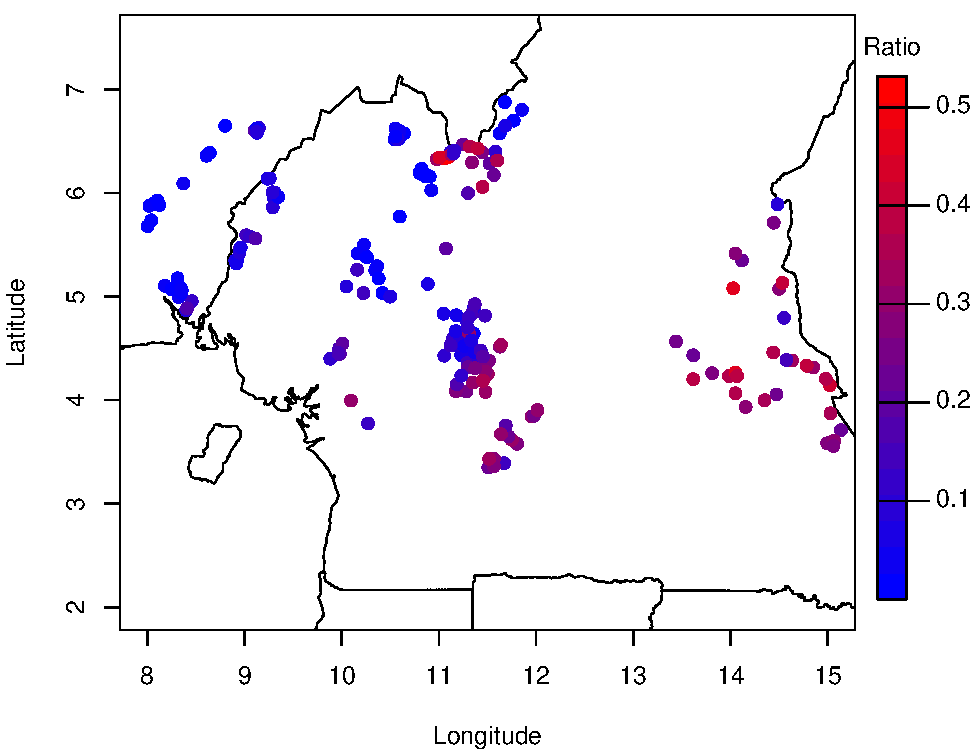
\includegraphics[width=.8\textwidth]{loaloa_ratio}  
\end{figure}
\end{frame}

\begin{frame}
\begin{figure}
\centering
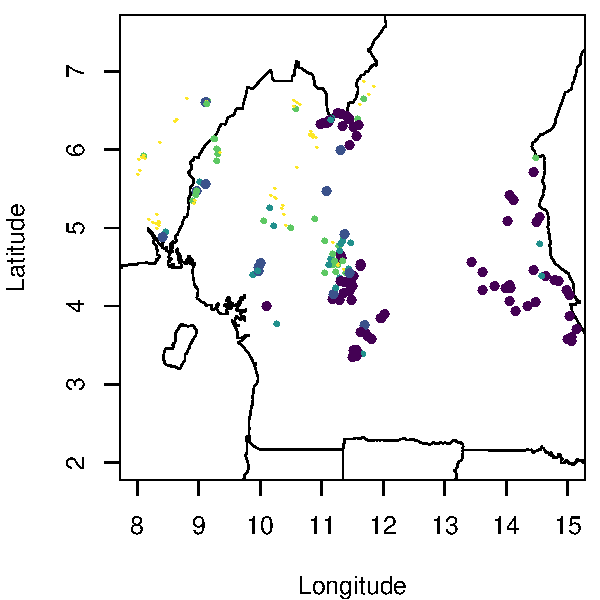
\includegraphics[width=.6\textwidth]{demo02} % 单图
\end{figure}
\end{frame}

\begin{frame}
\begin{figure}
\centering
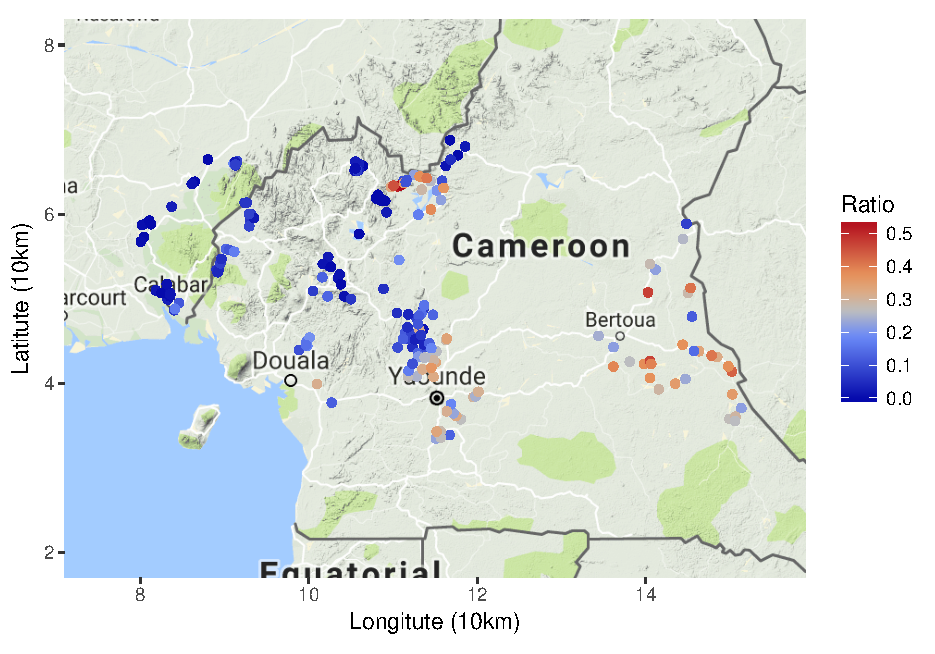
\includegraphics[width=.8\textwidth]{demo03} % 单图
\end{figure}
\end{frame}



\section{结论与展望}

\begin{frame}
\centering {\zihao{0} \color{red} \calligra{Thank You}}

\end{frame}



\begin{frame}[allowframebreaks]
\frametitle{References}
\scriptsize
\bibliographystyle{authordate1}
\bibliography{R-GLMM-pkgs}
\end{frame}

\appendix

\section*{附录}

\begin{frame}{Softwares and Tools}
\begin{figure}

\centering

\includegraphics[width=.2\textwidth]{software/r}\qquad

\includegraphics[width=.16\textwidth]{software/stan} \\ 

\includegraphics[width=.45\textwidth]{software/bioconductor}

\includegraphics[width=.45\textwidth]{software/PyMC3} 
\caption{{\color{OrangeRed1} GNU R} {\color{SpringGreen4} INLA}  {\color{OrangeRed1} Stan} {\color{SpringGreen4} PyMC3}}

\end{figure}
\end{frame}
%% OpenBUGS  WinBUGS  JAGS
% library(R2OpenBUGS) # 2017-2-20 version 3.2-3.2
% library(R2WinBUGS) # 2015-07-29 version 2.1-21
% library(rjags) # 2016-02-19 version 4-6
% library(BRugs) # OpenBUGS 2017-06-26  version 0.9-0
% library(glmmBUGS) # Generalised Linear Mixed Models with BUGS and JAGS 2016-09-22 version 2.4.0
% library(R2jags) # Using R to Run 'JAGS'  2015-08-23	 version 0.5-7

% network
	% diagram DiagrammeR DiagrammeRsvg
 % library(help=graph)

 % library(help=Rgraphviz)
 % library(help=igraph)

\begin{frame}{Projects}

\begin{figure}
\centering

\includegraphics[width=.3\textwidth]{software/GeoDa}\\

\includegraphics[width=.8\textwidth]{software/bioconductor}
\end{figure}

\end{frame}


\begin{frame}{Ack}
\begin{itemize}
\item[\faGithub] \href{https://github.com/Cloud2016}{Cloud2016} \faAt Github
\item[\aiOverleaf] \href{https://www.overleaf.com/}{Xiangyun} \faAt Overleaf
\item[\aiarXiv] \href{https://arxiv.org/}{arXiv}
\end{itemize}
\end{frame}

\end{document} 


